\chapter{Experiments}
\label{chap:experiments}

This chapter evaluates whether the graphon-based generative strategy implemented by OGAD can reproduce graph distributions arising from heterogeneous structural mechanisms. Rather than assessing the method on a single graph family, the experiments test whether an intermediate graphon representation can support generation across structurally different distributions. OGAD is compared with DiGress and classical probabilistic graph generators under the common evaluation framework introduced in Chapter~\ref{chap:method}.

The experimental analysis is organized around the three research questions introduced in Chapter~\ref{chap:introduction}. \textbf{RQ1} asks whether discrete diffusion over graphon-derived representations can generate graph distributions that preserve relevant structural properties across different graph families; \textbf{RQ2} examines how OGAD compares with direct graph diffusion and classical generators under the same evaluation protocol; and \textbf{RQ3} investigates whether the relative behavior of the compared methods remains consistent across structural descriptors and datasets.

Five synthetic graph families are selected to cover complementary structural regimes. Erd\H{o}s--R\'enyi (ER) represents homogeneous random connectivity; the Stochastic Block Model (SBM) introduces explicit community structure; Barab\'asi--Albert (BA) produces strong degree heterogeneity through preferential attachment; Watts--Strogatz (WS) captures small-world structure and local clustering; and the expected-degree graph family (EDG) introduces controlled heterogeneity through node-specific connection propensities. Their diversity is deliberate: together, these datasets provide a controlled test of the ability of the graphon-based representation to accommodate graph distributions generated by substantially different structural mechanisms.

Generated graph distributions are compared with held-out test graphs using Maximum Mean Discrepancy (MMD) over three structural descriptors: degree distribution, clustering-coefficient distribution, and normalized-Laplacian spectrum, following Section~\ref{sec:method_ggme}. Lower MMD values indicate closer agreement with the reference distribution. Raw MMD results are complemented by rank-based aggregations that summarize relative performance across datasets and structural descriptors.

\section{Experimental Setup}
\label{sec:exp_setup}

\subsection{Datasets}
\label{subsec:exp_datasets}

The evaluation uses five synthetic graph datasets, each containing \(300\) simple undirected graphs with \(n=100\) nodes.
The datasets were generated with master seed \(42\) and partitioned into \(240\) training graphs and \(60\) test graphs.
The final test set remains excluded from both model training and candidate selection, following Section~\ref{sec:method_input_partitioning}, and is accessed only during final evaluation.

A common graph size of \(n=100\) is used across all five families, keeping graph size fixed across datasets and allowing the comparison to focus on differences in structural organization.

The five datasets are generated according to distinct mechanisms.
Erd\H{o}s--R\'enyi (ER) graphs follow \(G(100,0.05)\), with each possible edge sampled independently with probability \(0.05\).
The Stochastic Block Model (SBM) contains four equally sized communities of \(25\) nodes, with within-community edge probability \(0.10\) and between-community probability \(0.01\).
Barab\'asi--Albert (BA) graphs are generated by preferential attachment with \(m=3\).
Watts--Strogatz (WS) graphs use \(k=8\) nearest neighbors and rewiring probability \(0.1\).
Finally, in the expected-degree graph family (EDG), node weights are independently sampled from \(\mathcal{U}(1,20)\), and edges are generated with probabilities

\[
p_{ij}
=
\min\left(
\frac{w_i w_j}{\sum_k w_k},
1
\right),
\qquad i \neq j,
\]

with self-loops excluded.

Table~\ref{tab:exp_datasets} summarizes the generation parameters and the empirical mean density of the training graphs.
\begin{table}[H]
    \centering
    \caption{Synthetic graph datasets used in the experimental evaluation.}
    \label{tab:exp_datasets}
    \begin{tabularx}{\textwidth}{l l l}
        \hline
        Dataset & Mean density & Main structural property \\
        \hline
        ER  & 0.049913 & homogeneous random connectivity \\
        SBM & 0.031775 & community structure \\
        BA  & 0.058788 & preferential attachment \\
        WS  & 0.080808 & small-world structure \\
        EDG & 0.105096 & heterogeneous expected degrees \\
        \hline
    \end{tabularx}
\end{table}

The suite therefore spans complementary structural regimes: homogeneous random connectivity in ER, explicit community organization in SBM, preferential-attachment-driven degree heterogeneity in BA, small-world organization and local clustering in WS, and heterogeneous connection propensities in EDG.
This diversity provides a controlled test of whether the graphon-based generative strategy can reproduce graph distributions arising from substantially different structural mechanisms.

\subsection{Compared Models}
\label{subsec:exp_models}

OGAD is compared with DiGress and four classical probabilistic graph generators:

\begin{itemize}
    \item \textbf{DiGress}, a discrete diffusion model operating directly in the graph domain;
    \item \textbf{Erd\H{o}s--R\'enyi (ER)}, fitted through a global edge probability;
    \item \textbf{Configuration Model}, based on degree information estimated from the training graphs;
    \item \textbf{Stochastic Block Model (SBM)}, based on community-dependent connection probabilities;
    \item \textbf{Degree-Corrected Stochastic Block Model (DC-SBM)}, which additionally models degree heterogeneity within communities.
\end{itemize}

All models are evaluated through the same GGME procedure, so the reported differences arise from the generated graph distributions rather than from model-specific evaluation criteria.


\subsection{Baseline Configuration}
\label{subsec:exp_baseline_configuration}

The classical baselines are fitted exclusively from the training graphs and generate \(100\) graphs for final evaluation. The ER baseline estimates a global edge probability; the Configuration Model samples degree sequences from pooled training-set degree information; the SBM baseline estimates community structure and block-level connection probabilities; and DC-SBM additionally introduces heterogeneous node-level degree effects.

Classical baseline generation uses random seed \(42\).

DiGress is trained using the CommunityGraphs configuration. The executed configuration uses \(200\) epochs, batch size \(32\), gradient accumulation over \(16\) batches, \(1000\) diffusion steps, \(8\) graph-transformer layers, and \(8\) attention heads. The final DiGress graph set evaluated by GGME contains \(100\) graphs.

Where possible, DiGress and the classical baselines are generated once per dataset and reused across the corresponding OGAD runs. Thus, different OGAD configurations are compared against the same baseline graph collections.


\subsection{OGAD Experimental Configuration}
\label{subsec:exp_ogad_configuration}

The OGAD processing stages are defined in Chapter~\ref{chap:method}. Table~\ref{tab:exp_fixed_parameters} reports the principal numerical settings used in the successful experiments.

\begin{table}[htbp]
    \centering
    \caption{Main fixed parameters used in the OGAD experiments.}
    \label{tab:exp_fixed_parameters}
    \begin{tabular}{ll}
        \hline
        Parameter & Value \\
        \hline
        Graphon resolution & \(128\times128\) \\
        SIGL epochs & \(100\) \\
        SIGL learning rate & \(0.06\) \\
        SIGL INR batch size & \(1024\) \\
        Bootstrap replicates & \(500\) \\
        Bootstrap seed & \(0\) \\
        SIGL workers & \(4\) \\
        D3PM hidden dimension & \(512\) \\
        D3PM batch size & \(32\) \\
        D3PM diffusion steps & \(1000\) \\
        D3PM maximum epochs & \(300\) \\
        Early-stopping patience & \(25\) \\
        Early-stopping minimum improvement & \(5\times10^{-5}\) \\
        D3PM train/validation split & \(80/20\) \\
        D3PM split seed & \(0\) \\
        Generated graphon tensors per candidate & \(16\) \\
        Generated graphs per evaluation & \(100\) \\
        GGME seed & \(0\) \\
        \hline
    \end{tabular}
\end{table}

The main experimentally varied quantities are the number of clusters used before the SIGL bootstrap procedure and the hyperparameters defining each D3PM candidate configuration.

The principal sweep uses requested cluster counts

\[
C_{\mathrm{req}}\in\{1,4,8,12,16\}.
\]

As explained in Section~\ref{subsec:method_sigl_clustering}, the requested number of clusters can differ from the number of effective non-empty clusters obtained at runtime.

For each complete run in the main sweep, the D3PM candidate grid is defined by

\[
\eta
\in
\left\{
2\times10^{-5},
3\times10^{-5},
5\times10^{-5}
\right\},
\qquad
K\in\{8,10,12,14,16\},
\qquad
\lambda\in\{0.006,0.01\},
\]

resulting in twelve candidate configurations per OGAD run.

Additional follow-up experiments were performed for BA and WS using

\[
C_{\mathrm{req}}\in\{4,8,16\},
\]

and

\[
\eta
\in
\left\{
1\times10^{-5},
2\times10^{-5},
3\times10^{-5}
\right\},
\qquad
K\in\{10,14\},
\qquad
\lambda=0.006,
\]

resulting in six D3PM candidate configurations per run.


\subsection{Training and Candidate Selection}
\label{subsec:exp_candidate_selection}

The selection procedure follows the distinction introduced in Section~\ref{sec:method_d3pm_selection} between checkpoint selection within one D3PM candidate and generator selection across candidate configurations.

The \(240\) training graphs are first partitioned, using an \(80/20\) split with seed \(0\), into

\[
|\mathcal{G}_{\mathrm{model}}|=192
\]

graphs used by SIGL and

\[
|\mathcal{G}_{\mathrm{GGME-val}}|=48
\]

graphs reserved for graph-domain candidate validation.

The graphon collection produced by SIGL is independently divided into D3PM training and validation subsets, again using an \(80/20\) split with seed \(0\).

For each D3PM candidate configuration, training retains the checkpoint with the lowest validation loss. The retained checkpoint is then used to generate \(16\) graphon-like tensors, which are converted into finite graphs through the procedure described in Section~\ref{sec:method_graph_sampling}.

The graph distribution generated by each candidate is compared against \(\mathcal{G}_{\mathrm{GGME-val}}\) using GGME. The candidate obtaining the best GGME validation result according to the configured selection rule is retained as the selected D3PM candidate for that OGAD run.

The procedure can therefore be summarized as

\[
\begin{gathered}
\text{D3PM candidate}
\longrightarrow
\text{best checkpoint within candidate}
\longrightarrow
\text{generated graphs}
\\[0.4em]
\longrightarrow
\text{GGME validation}
\longrightarrow
\text{selected candidate}.
\end{gathered}
\]

The first selection operates in graphon representation space through the D3PM validation objective, whereas the second operates directly in graph space through GGME. The final test/reference graphs do not participate in either selection stage.


\subsection{Experimental Campaign and Completed Runs}
\label{subsec:exp_campaign}

The final experiments were obtained through a main broad sweep over all five datasets and a subsequent follow-up focused on BA and WS.

% \begin{table}[htbp]
%     \centering
%     \caption{Main experimental sweeps contributing to the final evaluation.}
%     \label{tab:exp_campaigns}
%     \begin{tabular}{llll}
%         \hline
%         Sweep & Datasets & Cluster counts & D3PM learning rates \\
%         \hline
%         Main & ER, SBM, BA, WS, EDG
%         & \(1,4,8\)
%         & \(2,3,5\times10^{-5}\) \\
%         Follow-up & BA, WS
%         & \(4,8,16\)
%         & \(1,2,3\times10^{-5}\) \\
%         \hline
%     \end{tabular}
% \end{table}

Only runs completing all stages required for final GGME evaluation are included in the analysis. Exploratory executions are excluded from the quantitative comparison.

% \begin{table}[htbp]
%     \centering
%     \caption{Complete OGAD runs containing all three final GGME descriptor evaluations.}
%     \label{tab:exp_complete_runs}
%     \begin{tabular}{lc}
%         \hline
%         Dataset & Complete runs \\
%         \hline
%         ER  & 7 \\
%         SBM & 6 \\
%         BA  & 6 \\
%         WS  & 4 \\
%         EDG & 6 \\
%         \hline
%     \end{tabular}
% \end{table}



\subsection{Evaluation Protocol}
\label{subsec:exp_evaluation}

Final evaluation follows Section~\ref{sec:method_ggme}. For every evaluated model, \(100\) generated graphs are compared with the held-out test graph distribution through:

\begin{enumerate}
    \item degree distribution (DD);
    \item clustering-coefficient distribution (CC);
    \item normalized-Laplacian spectrum (NL).
\end{enumerate}

For dataset \(D\), descriptor \(d\), and model \(m\), let

\[
M_{D,d}(m)
\]

denote the corresponding MMD value. Lower values indicate closer agreement between the generated and reference descriptor distributions.

A small number of reported MMD values are slightly negative. These values are retained exactly as emitted by the evaluation implementation, and ranking follows their reported numerical ordering.


\subsection{Aggregate Rank Analysis}
\label{subsec:exp_rank_method}

Raw MMD values cannot be meaningfully averaged across DD, CC, and NL because the descriptors operate on different representations and numerical scales. A rank-based analysis is therefore used as a complementary summary.

For every dataset \(D\), descriptor \(d\), and model \(m\), let

\[
r_{D,d}(m)\in\{1,\ldots,6\}
\]

be the rank obtained by sorting models by increasing MMD, with rank \(1\) assigned to the best result. Exact ties receive the average of the occupied ranks.

The first aggregation computes the mean rank across datasets for each descriptor:

\[
\overline{r}_{d}(m)
=
\frac{1}{5}
\sum_{D\in\mathcal{D}}
r_{D,d}(m),
\]

where

\[
\mathcal{D}
=
\{
\mathrm{ER},
\mathrm{SBM},
\mathrm{BA},
\mathrm{WS},
\mathrm{EDG}
\}.
\]

The second computes the mean rank across descriptors for each dataset:

\[
\overline{r}_{D}(m)
=
\frac{1}{3}
\sum_{d\in\{\mathrm{DD},\mathrm{CC},\mathrm{NL}\}}
r_{D,d}(m).
\]

Lower mean ranks are better in both cases.

\section{Quantitative Results}
\label{sec:exp_results}

Tables~\ref{tab:exp_er}--\ref{tab:exp_edg} report the MMD values obtained on the five graph families for degree distribution (DD), clustering-coefficient distribution (CC), and normalized-Laplacian spectrum (NL).
Lower values indicate closer agreement with the reference distribution, and the best result for each descriptor is highlighted in bold.

\begin{table}[H]
    \centering
    \caption{MMD results on the Erd\H{o}s--R\'enyi dataset.}
    \label{tab:exp_er}
    \begin{tabular}{lrrr}
        \hline
        Model & DD & CC & NL \\
        \hline
        OGAD          & 0.080129 & 69.4112   & \(4.288\times10^{-6}\) \\
        DiGress       & 0.007058 & 21.5956   & \(\mathbf{-1.101\times10^{-6}}\) \\
        ER            & \textbf{0.001205} & \textbf{-4.56225} & \(5.754\times10^{-7}\) \\
        Configuration & 0.001266 & 7.37291   & \(-6.987\times10^{-7}\) \\
        SBM           & 0.004082 & 927.725   & \(2.563\times10^{-6}\) \\
        DC-SBM        & 0.161066 & 1291.50   & \(1.178\times10^{-5}\) \\
        \hline
    \end{tabular}
\end{table}

On ER, the matched probabilistic baseline yields the lowest discrepancies for degree and clustering, while DiGress performs best on the spectral descriptor.
OGAD is comparatively weaker across all three descriptors, illustrating the advantage of a generator whose assumptions directly match the target distribution.

\begin{table}[H]
    \centering
    \caption{MMD results on the Stochastic Block Model dataset.}
    \label{tab:exp_sbm}
    \begin{tabular}{lrrr}
        \hline
        Model & DD & CC & NL \\
        \hline
        OGAD          & 0.016365 & \textbf{0.203109} & \(4.035\times10^{-7}\) \\
        DiGress       & \textbf{0.002235} & 190.035 & \(1.005\times10^{-6}\) \\
        ER            & 0.003837 & 430.763 & \(\mathbf{-1.774\times10^{-7}}\) \\
        Configuration & 0.003710 & 614.534 & \(1.609\times10^{-8}\) \\
        SBM           & 0.014688 & 695.475 & \(1.962\times10^{-6}\) \\
        DC-SBM        & 0.217106 & 1394.32 & \(3.628\times10^{-6}\) \\
        \hline
    \end{tabular}
\end{table}

On SBM, OGAD achieves the lowest clustering discrepancy by a substantial margin, whereas DiGress performs best on degree distribution and ER on the spectral descriptor.
The result highlights a marked strength of OGAD in reproducing clustering structure without a corresponding advantage on all descriptors.

\begin{table}[H]
    \centering
    \caption{MMD results on the Barab\'asi--Albert dataset.}
    \label{tab:exp_ba}
    \begin{tabular}{lrrr}
        \hline
        Model & DD & CC & NL \\
        \hline
        OGAD          & 0.980363 & 508.541 & \(3.543\times10^{-5}\) \\
        DiGress       & 0.204514 & \textbf{78.0936} & \(\mathbf{1.979\times10^{-6}}\) \\
        ER            & 1.137100 & 1821.88 & \(1.337\times10^{-5}\) \\
        Configuration & \textbf{0.008423} & 900.171 & \(1.302\times10^{-5}\) \\
        SBM           & 1.135680 & 968.017 & \(1.524\times10^{-5}\) \\
        DC-SBM        & 0.882699 & 381.599 & \(1.777\times10^{-5}\) \\
        \hline
    \end{tabular}
\end{table}

BA is a more challenging setting for OGAD.
The Configuration Model provides the closest degree match, while DiGress obtains the lowest discrepancies for both clustering and spectrum.

\begin{table}[H]
    \centering
    \caption{MMD results on the Watts--Strogatz dataset.}
    \label{tab:exp_ws}
    \begin{tabular}{lrrr}
        \hline
        Model & DD & CC & NL \\
        \hline
        OGAD          & 0.333326 & 2221.89 & \(1.290\times10^{-4}\) \\
        DiGress       & 0.290017 & \textbf{1505.24} & \(\mathbf{9.620\times10^{-5}}\) \\
        ER            & 0.322729 & 4532.93 & \(1.890\times10^{-4}\) \\
        Configuration & \textbf{0.040790} & 6003.34 & \(1.880\times10^{-4}\) \\
        SBM           & 0.297014 & 2783.35 & \(1.910\times10^{-4}\) \\
        DC-SBM        & 0.314288 & 2758.55 & \(1.860\times10^{-4}\) \\
        \hline
    \end{tabular}
\end{table}

On WS, OGAD is second only to DiGress for both clustering and spectral similarity, but performs poorly on degree distribution.
This contrast again shows that agreement on local and spectral structure does not necessarily imply an accurate degree match.

\begin{table}[H]
    \centering
    \caption{MMD results on the expected-degree graph dataset.}
    \label{tab:exp_edg}
    \begin{tabular}{lrrr}
        \hline
        Model & DD & CC & NL \\
        \hline
        OGAD          & 0.022283 & \textbf{20.871} & \(1.696\times10^{-5}\) \\
        DiGress       & 0.020852 & 58.5847 & \(\mathbf{6.623\times10^{-6}}\) \\
        ER            & 0.519254 & 1397.30 & \(5.101\times10^{-5}\) \\
        Configuration & 0.022298 & 87.0578 & \(1.614\times10^{-5}\) \\
        SBM           & 0.355204 & 736.207 & \(1.326\times10^{-5}\) \\
        DC-SBM        & \textbf{0.012818} & 127.286 & \(5.929\times10^{-5}\) \\
        \hline
    \end{tabular}
\end{table}

EDG is the most favorable setting for OGAD among the five datasets.
OGAD achieves the lowest clustering discrepancy and a degree-distribution result close to DiGress and the Configuration Model, although DiGress remains stronger on the spectral descriptor.

\subsection{Qualitative Examples of Generated Graphs and Graphons}
\label{subsec:qualitative_examples}

The quantitative evaluation is complemented by a qualitative inspection of
representative high- and low-performing OGAD runs. The label above each
reference graph identifies the dataset: \texttt{sbm\_n100\_4c} denotes a
100-node stochastic block model with four communities,
\texttt{expdeg\_n100\_lin} a 100-node expected-degree model with a linear
degree profile, and \texttt{er\_n100\_p005} a 100-node Erd\H{o}s--R\'enyi
model with $p=0.05$. The label above each generated graph is the identifier
of the corresponding experimental run; in particular, the final
\texttt{ncX} component is a run/configuration identifier and should not be
interpreted directly as the number of clusters, which is reported separately
as \texttt{nc} in the statistics.

For each run, the annotations report its average rank over the three GGME
descriptors, the MMD values for degree distribution, clustering coefficient,
and normalized Laplacian spectrum, together with the density and clustering
coefficient of the target and displayed generated graph. The graphon mean and
standard deviation summarize the generated probability surface. In the
graphon heatmaps, dark purple denotes low edge probability and progressively
lighter blue--green regions denote higher probability; the dark main diagonal
corresponds to the enforced zero diagonal. The displayed graphon is the mean
of the generated graphon tensors and does not necessarily coincide with the
specific tensor from which the displayed graph was sampled.

\begin{figure}[H]
    \centering
    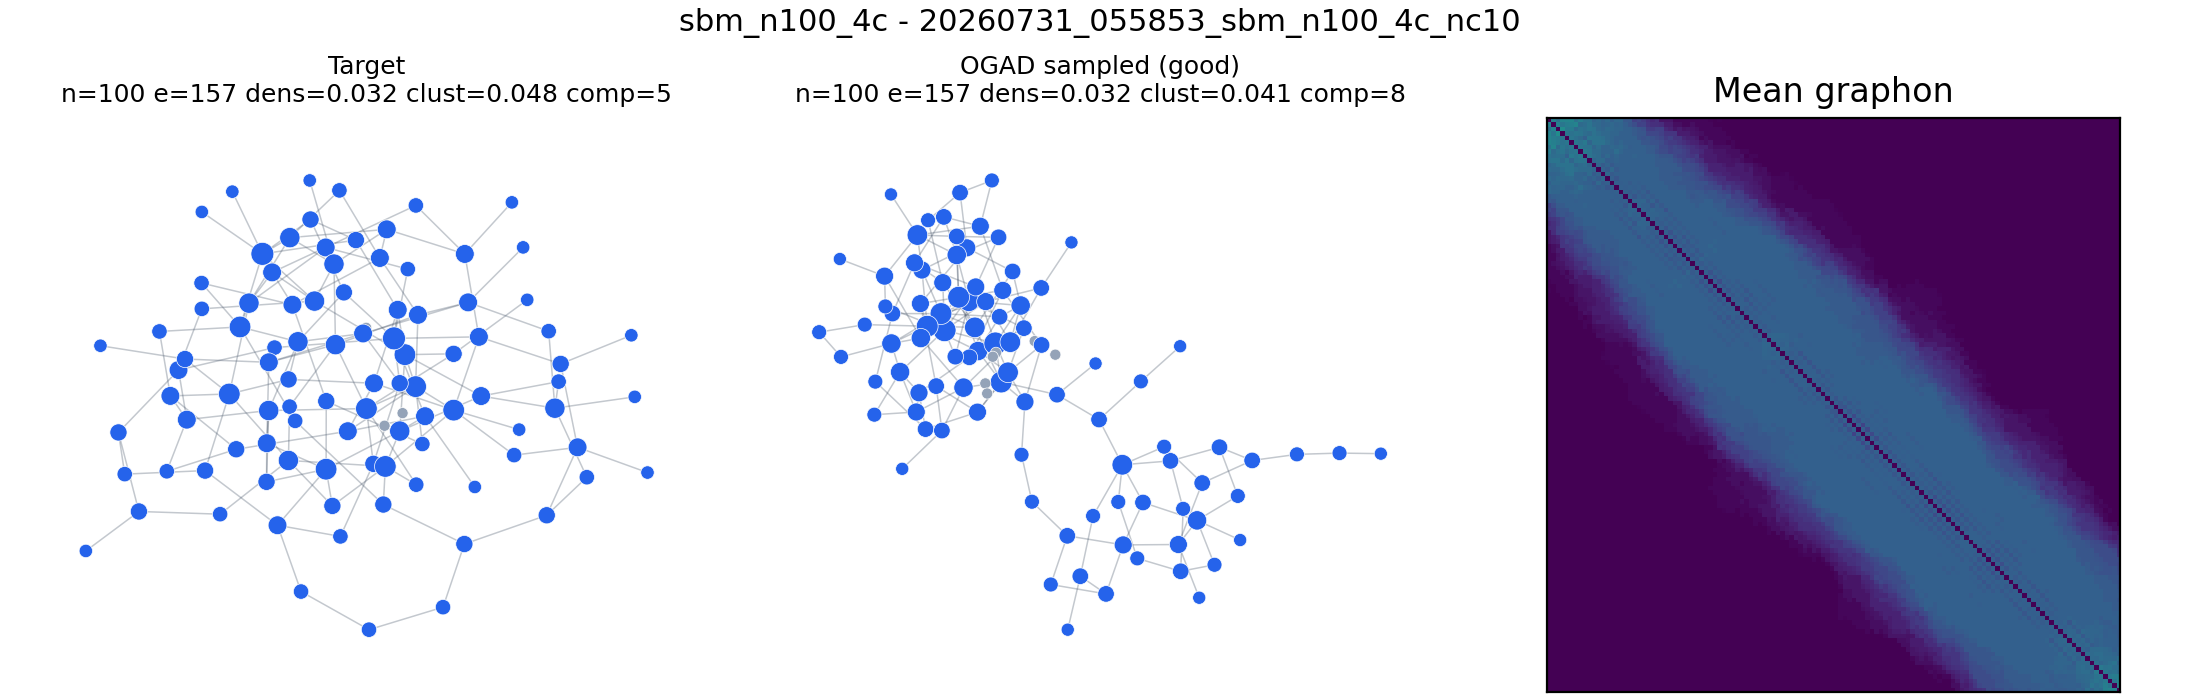
\includegraphics[width=\textwidth]
        {figures/experiments/good_sbm.png}

    \vspace{0.3em}

    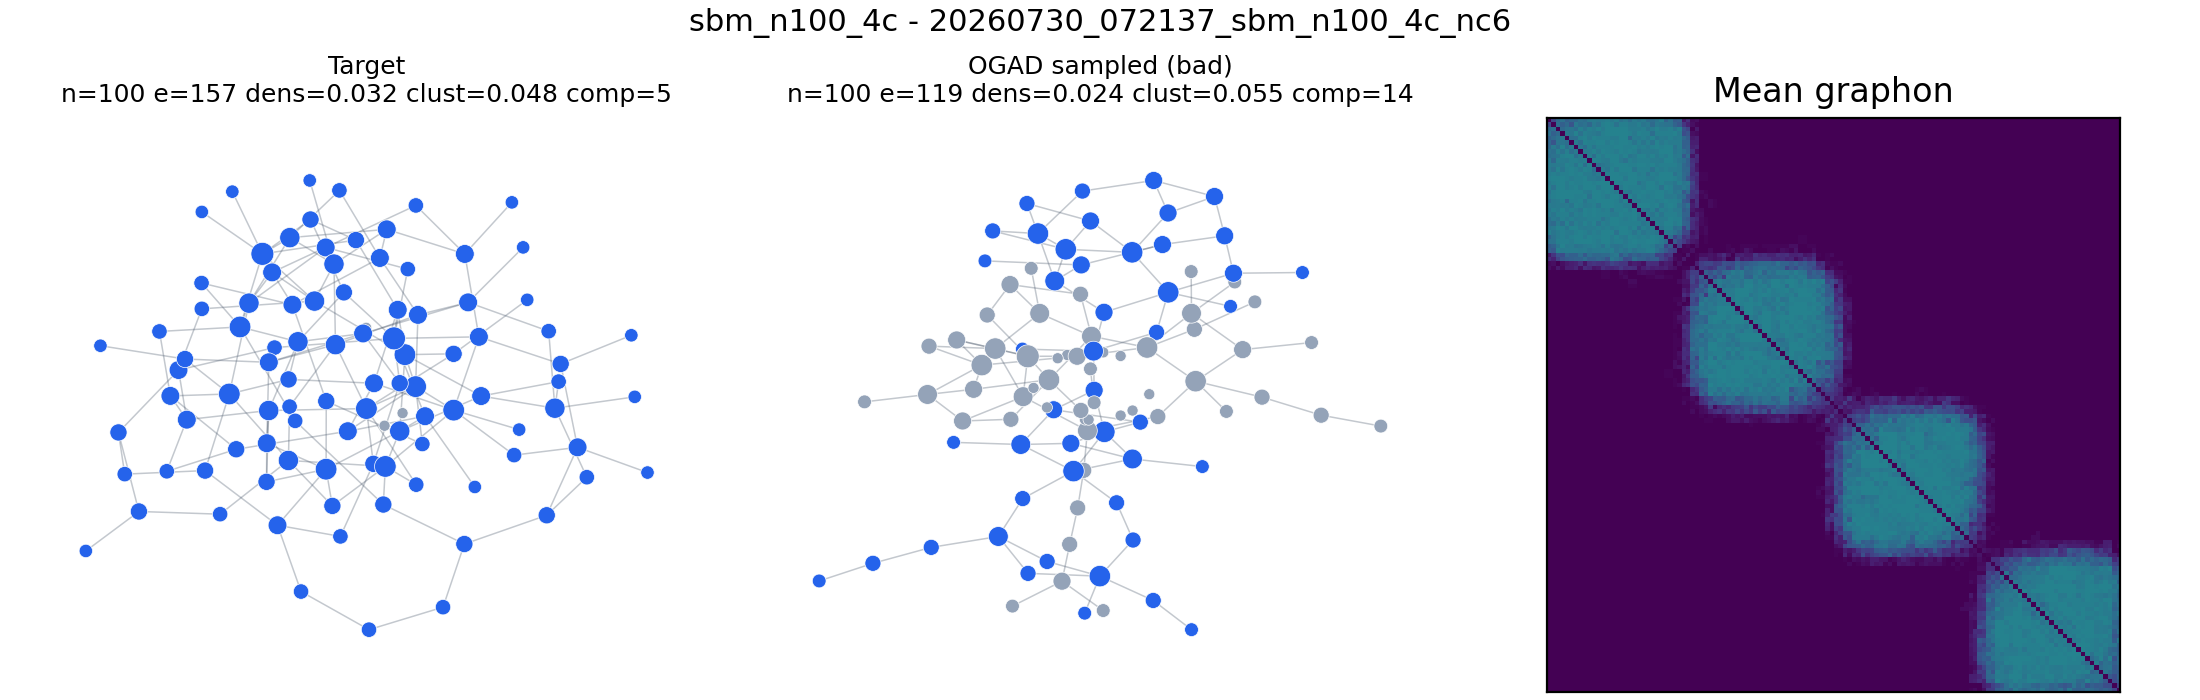
\includegraphics[width=\textwidth]
        {figures/experiments/bad_sbm.png}

    \caption{
        High- and low-performing OGAD runs on the SBM dataset.
        The high-performing run obtains MMD values of
        $0.0164$ (degree), $0.2031$ (clustering), and
        $4.04\times10^{-7}$ (normalized Laplacian spectrum),
        whereas the low-performing run obtains
        $0.278$, $54.01$, and $3.23\times10^{-6}$, respectively.
        Although the low-performing graphon exhibits a visually pronounced block
        structure, its generated graph distribution is substantially less faithful
        according to all three descriptors.
    }
    \label{fig:qual_sbm}
\end{figure}

\begin{figure}[H]
    \centering
    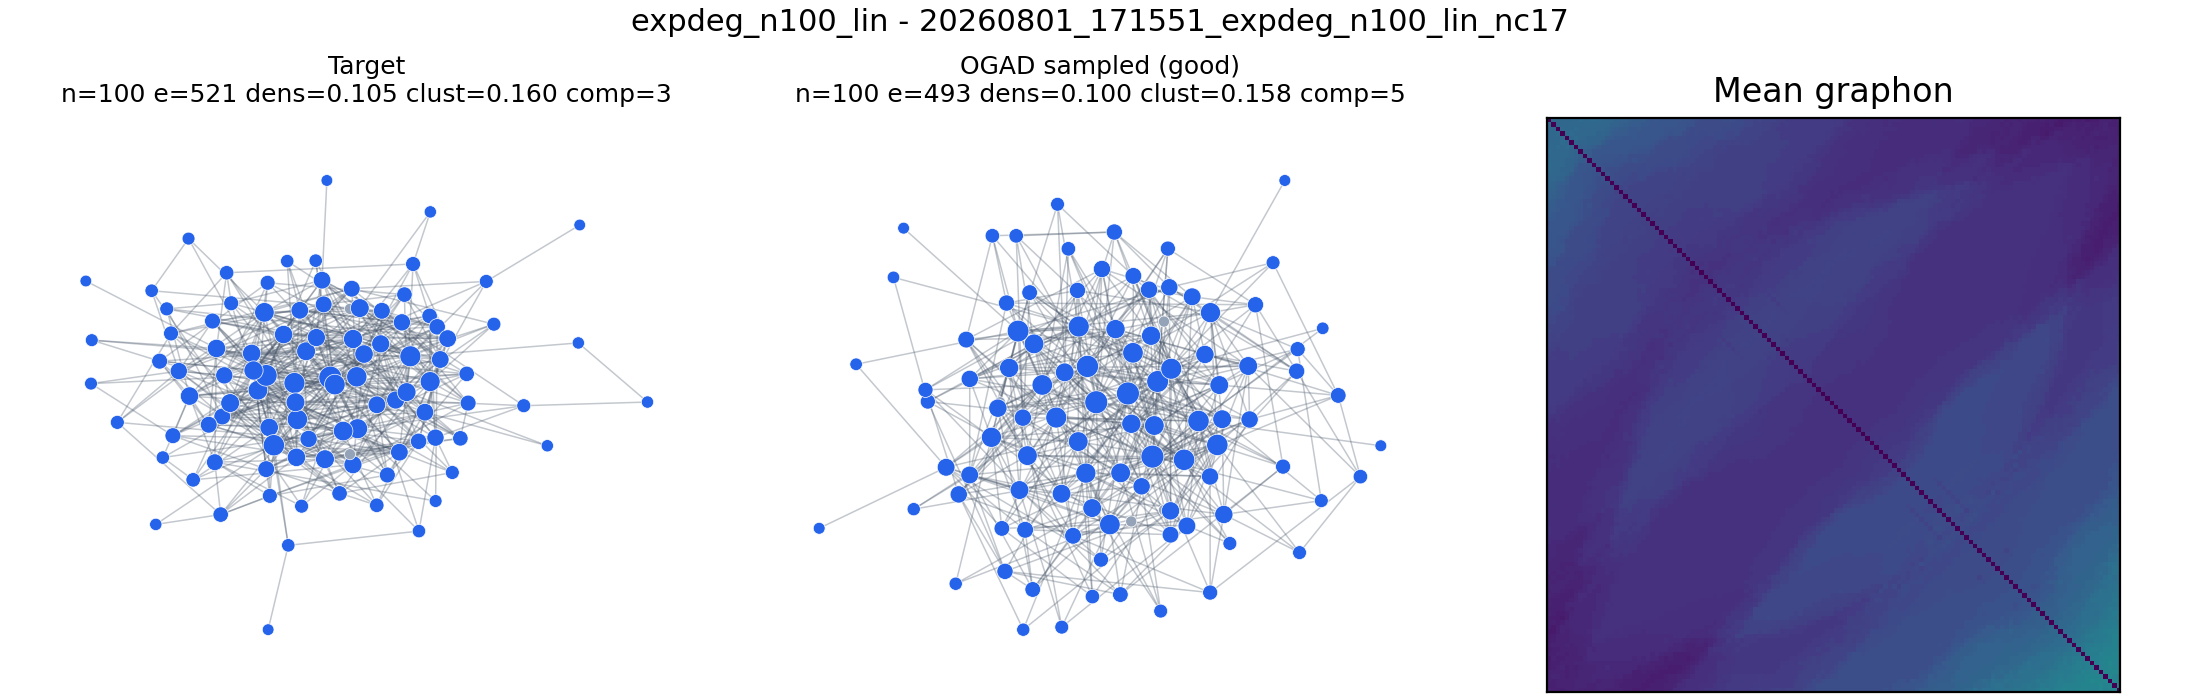
\includegraphics[width=\textwidth]
        {figures/experiments/good_expdeg.png}

    \vspace{0.3em}

    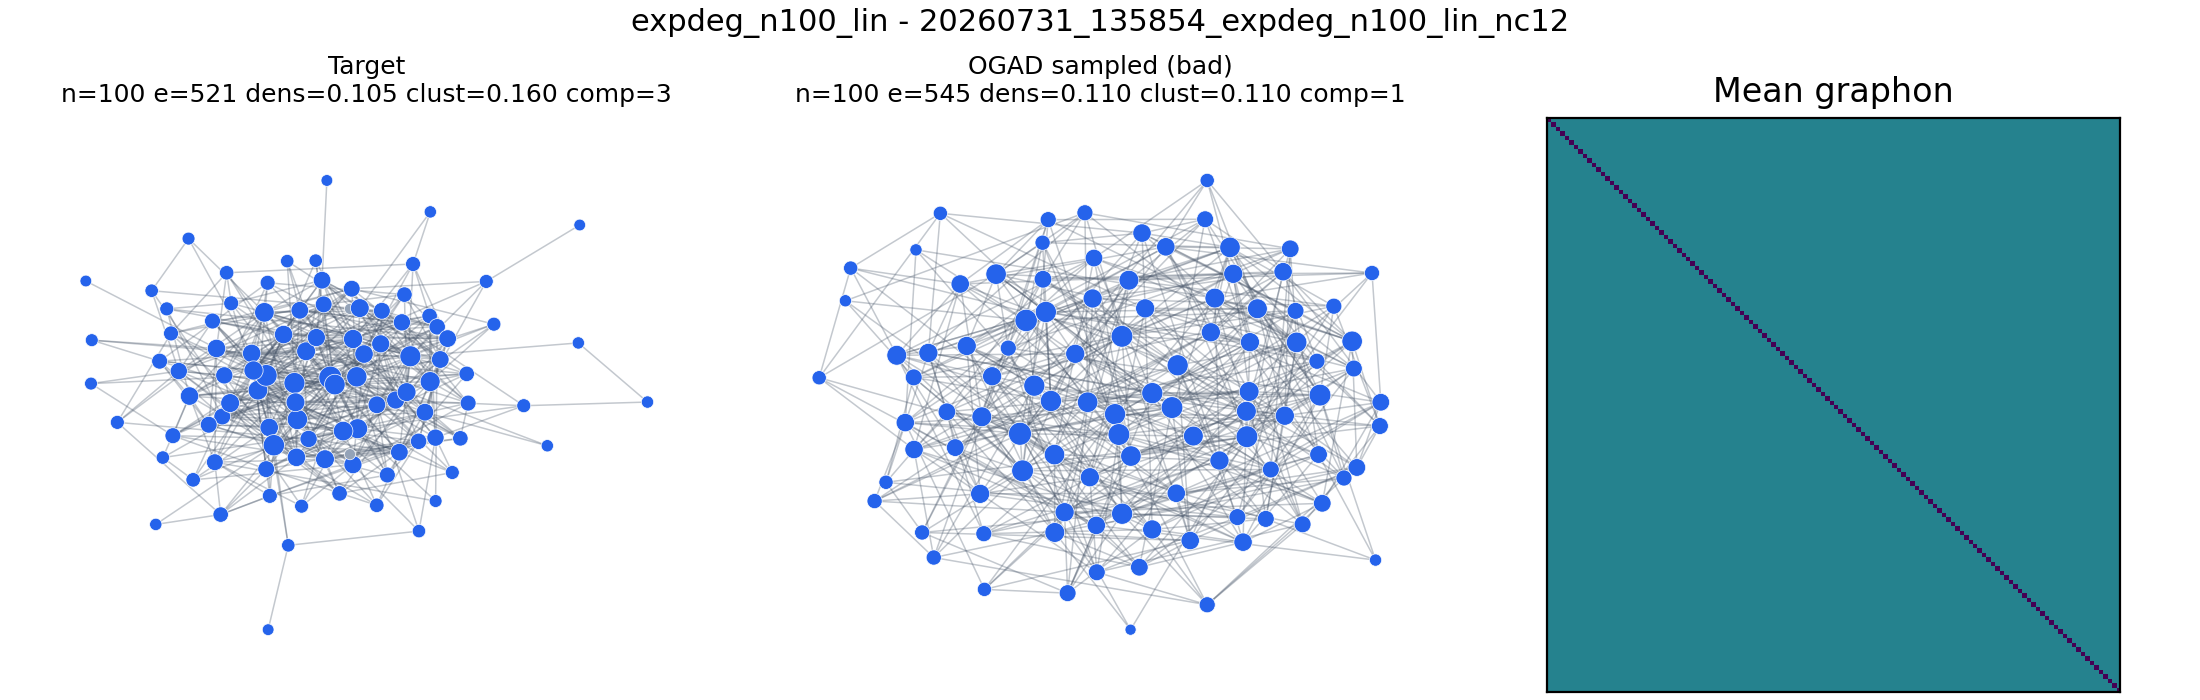
\includegraphics[width=\textwidth]
        {figures/experiments/bad_expdeg.png}

    \caption{
        High- and low-performing OGAD runs on the expected-degree dataset.
        The high-performing run obtains MMD values of
        $0.0223$ (degree), $20.87$ (clustering), and
        $2.59\times10^{-5}$ (normalized Laplacian spectrum),
        whereas the low-performing run obtains
        $0.504$, $1494$, and $4.68\times10^{-5}$, respectively.
        The high-performing graphon better preserves the heterogeneous probability
        structure expected from the node-dependent degree profile, while the
        low-performing graphon approaches an almost uniform surface, consistently
        with the strong degradation in degree and clustering statistics.
    }
    \label{fig:qual_edg}
\end{figure}

\begin{figure}[H]
    \centering
    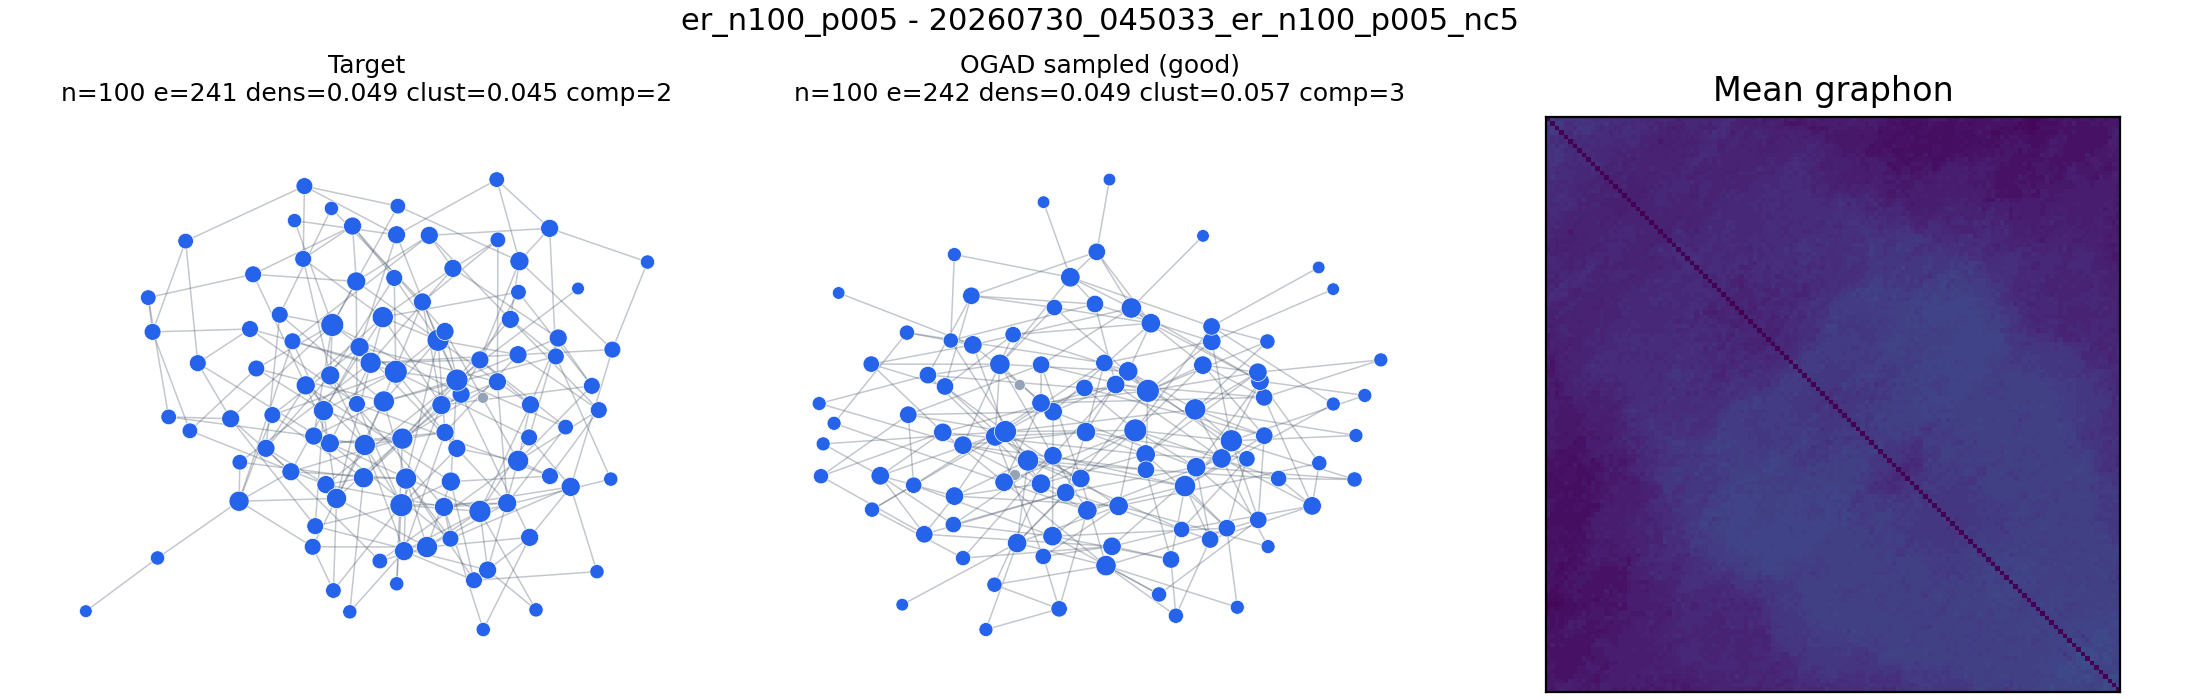
\includegraphics[width=\textwidth]
        {figures/experiments/good_er.png}

    \vspace{0.3em}

    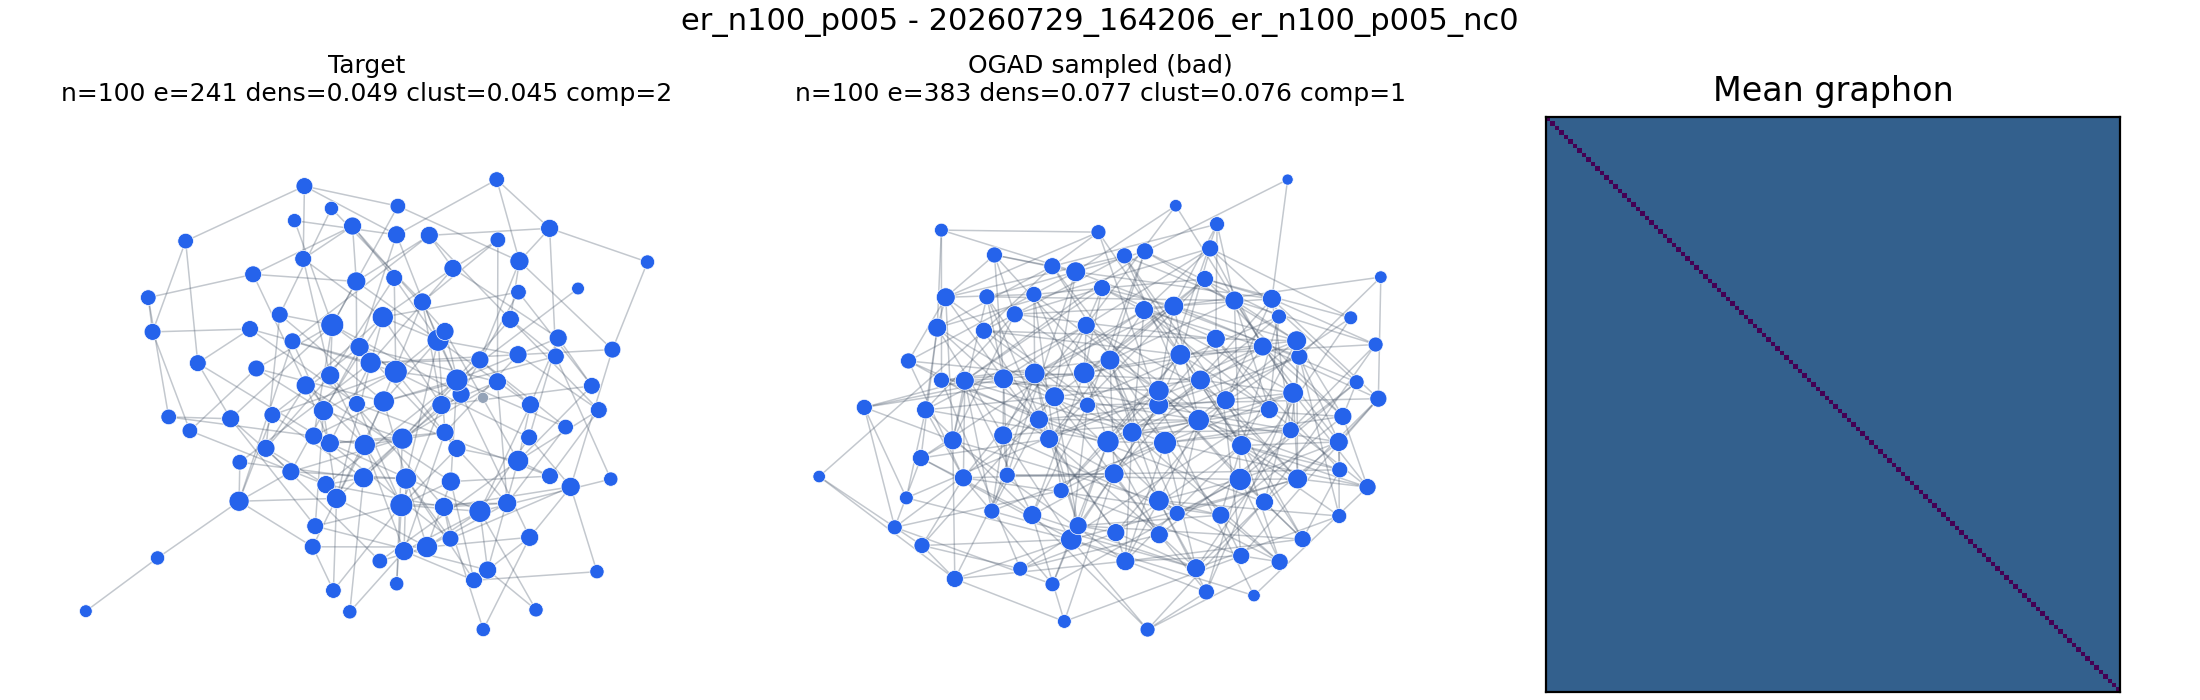
\includegraphics[width=\textwidth]
        {figures/experiments/bad_er.png}

    \caption{
        High- and low-performing OGAD runs on the Erd\H{o}s--R\'enyi dataset.
        The high-performing run obtains MMD values of
        $0.126$ (degree), $171.4$ (clustering), and
        $5.39\times10^{-6}$ (normalized Laplacian spectrum),
        whereas the low-performing run obtains
        $0.765$, $6272$, and $5.96\times10^{-5}$, respectively.
        Both graphons are approximately homogeneous, as expected for
        $G(n,p)$, but the low-performing run learns an excessively high
        edge-probability level, producing graphs that are substantially denser
        than the target.
    }
    \label{fig:qual_er}
\end{figure}

Overall, the examples are consistent with the distributional evaluation and
highlight different behaviors of the graphon-based representation: loss of
connectivity heterogeneity for the expected-degree model, incorrect probability
calibration for Erd\H{o}s--R\'enyi, and a possible discrepancy between visual
block structure and distribution-level fidelity for SBM. The quantitative MMD
evaluation therefore remains the primary basis for comparison, while these
visualizations provide complementary qualitative evidence.

\section{Aggregate Analysis and Discussion}
\label{sec:exp_rank_analysis}

The raw MMD values quantify descriptor-level discrepancies, while rank aggregation provides a scale-independent view of relative performance across datasets and structural properties.
The two analyses are therefore interpreted jointly.

\begin{table}[htbp]
    \centering
    \caption{Mean rank across the five datasets, computed separately for each descriptor. Lower is better.}
    \label{tab:exp_rank_metric}
    \begin{tabular}{lccc}
        \hline
        Model & DD & CC & NL \\
        \hline
        OGAD          & 4.60 & 2.20 & 4.00 \\
        DiGress       & 2.20 & \textbf{1.80} & \textbf{1.60} \\
        ER            & 4.20 & 4.20 & 3.40 \\
        Configuration & \textbf{2.00} & 3.80 & 2.60 \\
        SBM           & 4.00 & 4.80 & 4.20 \\
        DC-SBM        & 4.00 & 4.20 & 5.20 \\
        \hline
    \end{tabular}
\end{table}

Across datasets, clustering coefficient is the strongest descriptor for OGAD, with a mean rank of \(2.20\), compared with \(4.60\) for degree distribution and \(4.00\) for normalized-Laplacian spectrum.
This reflects the strong clustering results observed on SBM and EDG and the second-best result on WS.
The Configuration Model achieves the best average degree rank, while DiGress provides the most consistent spectral performance.

\begin{table}[htbp]
    \centering
    \caption{Mean rank across the three structural descriptors, computed separately for each dataset. Lower is better.}
    \label{tab:exp_rank_dataset}
    \begin{tabular}{lccccc}
        \hline
        Model & ER & SBM & BA & WS & EDG \\
        \hline
        OGAD          & 4.67 & 3.00 & 4.33 & 3.33 & 2.67 \\
        DiGress       & 2.67 & \textbf{2.33} & \textbf{1.33} & \textbf{1.33} & \textbf{1.67} \\
        ER            & \textbf{1.67} & \textbf{2.33} & 5.00 & 5.00 & 5.67 \\
        Configuration & 2.00 & 2.67 & 2.33 & 3.67 & 3.33 \\
        SBM           & 4.00 & 4.67 & 4.67 & 4.33 & 4.00 \\
        DC-SBM        & 6.00 & 6.00 & 3.33 & 3.33 & 3.67 \\
        \hline
    \end{tabular}
\end{table}

At dataset level, OGAD performs most favorably on EDG and SBM, with mean ranks of \(2.67\) and \(3.00\), respectively, while BA and ER are the most challenging settings.
DiGress is more consistent across the complete suite, whereas the classical generators are particularly competitive when their assumptions align with the target structure or descriptor, as illustrated by the matched ER baseline on ER and the Configuration Model on degree distribution.

Taken together, the MMD and rank results show a descriptor- and dataset-dependent behavior rather than a uniform advantage for OGAD.
Its most consistent empirical strength concerns clustering structure, particularly on SBM and EDG, whereas degree distribution and normalized-Laplacian similarity are reproduced less consistently.
The comparison with DiGress is especially informative because the two approaches apply discrete diffusion to different representations: directly to graph structure in DiGress and to categorical graphon representations in OGAD.
The observed results suggest that these representations favor different structural properties, although the experiments do not isolate which stage of the OGAD pipeline is responsible for the differences.


\section{Experimental Limitations}
\label{sec:exp_limitations}

The evaluation is restricted to synthetic graph families with \(100\) nodes and therefore does not establish performance on larger or real-world graph distributions.
The experimental search is not perfectly homogeneous across datasets, since BA and WS received additional follow-up exploration and the number of completed runs differs across graph families.
Moreover, degree distribution, clustering coefficient, and normalized-Laplacian spectrum capture complementary but incomplete aspects of graph structure.
Rank aggregation facilitates comparison across descriptors with different MMD scales but removes information about discrepancy magnitude and should therefore be interpreted together with the raw MMD values.
Only runs for which all three final GGME evaluations were completed are included in the reported comparison.